%! Mode:: "TeX:UTF-8"
%! TEX program = xelatex
\PassOptionsToPackage{quiet}{xeCJK}
\documentclass[withoutpreface,bwprint]{cumcmthesis}
\usepackage{etoolbox}
\BeforeBeginEnvironment{tabular}{\zihao{-5}}
\usepackage[numbers,sort&compress]{natbib}  % 文献管理宏包
\usepackage[framemethod=TikZ]{mdframed}  % 框架宏包
\usepackage{url}  % 网页链接宏包
\usepackage{subcaption}  % 子图宏包
\newcolumntype{C}{>{\centering\arraybackslash}X}
\newcolumntype{R}{>{\raggedleft\arraybackslash}X}
\newcolumntype{L}{>{\raggedright\arraybackslash}X}
\usepackage{amsmath}
\usepackage{graphicx}  % 用于 resizebox
\usepackage{booktabs} % 三线表宏包
\usepackage{siunitx}  % 数字对齐
\usepackage{tabularx}
\usepackage{float}
\usepackage{array}      % 列格式扩展
\usepackage{multirow}   % 多行合并

\title{破解校园单车潮汐:数据驱动与智能调度实践}  % 论文标题


%%%%%%%%%%%%%%%%%%%%%%%%%%%%%%%%%%%%%%%%%%%%%%%%%%%%%%%%%%%%%
%% 正文
\begin{document}

\maketitle
\begin{abstract}
共享单车作为高校短途出行的重要载体,长期面临"课表驱动型"潮汐需求与空间分布失配的双重挑战。本研究通过融合时空数据分析与智能优化算法,构建动态调度模型与点位布局策略,有效破解高峰时段供需失衡、车辆滞留及故障管理难题。

\textbf{对于问题一的单车总量估计与数量分布,}针对数据存在缺失值和时间间隔不均的问题,本文首先提出了一种基于时间段一致性与停车点功能类别相似性相结合的\textbf{均值填补与同类型点位趋势估算方法}处理缺失值。在此基础上,为解决仅有停车点数据而无法直接获知骑行中车辆数的问题,创新性地引入了随时间变化的\textbf{调整因子$\lambda_t$},结合\textbf{最小二乘法和K-means聚类算法}优化流动性调整因子,估算单车总量为\textbf{972}辆;通过\textbf{三次样条插值法}对填补和均值化处理后的数据进行拟合,生成了各停车点在指定时间点的车辆数分布,克服了原始数据时间点稀疏的问题,为后续分析提供了完整的时间序列数据。

\textbf{对于问题二的用车需求预测与调度模型,}定义租用需求为停车量差值,采用\textbf{XGBoost算法}预测需求,综合考虑了\textbf{时间、空间及KNN邻居相关性}等特征。基于预测的需求,为实现供需平衡,本文创新性地提出了\textbf{CVRPTC-SA优化算法(基于模拟退火的复杂VRP问题算法)}。人机交互地进行半自动化坐标提取,结合\textbf{Dijkstra 算法计算}最短路网距离,并采用\textbf{CVRPTC-SA算法}对 3 辆调度车的调度路径进行优化,目标为最小化总调度时间。结果生成了各时间段内满足约束的可行调度方案,有效缓解了潮汐效应。

\textbf{对于问题三的运营效率评价与点位布局优化,}本文构建\textbf{时间-空间网络流模型},运用\textbf{线性规划(Gurobi)}优化调度,以\textbf{最小化总调度成本(时间)和供需不平衡惩罚}为目标,综合评估\textbf{调度效率、需求满足率与点位利用率},构建了\textbf{综合运营效率评价函数},计算得初始运营效率为\textbf{0.7392},表明存在优化空间。通过迭代优化点位布局(移除校医院、体育馆,新增教学食堂结合部、一田右侧两个点位),最终优化后效率提升至\textbf{0.8588},增幅达\textbf{16.18\%},有效改善了高峰期供需矛盾。

\textbf{对于问题四的故障车辆处理,}在问题三优化后的点位布局基础上,针对\textbf{6\%} 的故障率,沿用\textbf{CVRPTC-SA 模型},优化了 3 辆运维车的巡检路线。模型综合考虑了\textbf{路径连续性、车辆容量及时间约束},成功回收全部故障车辆(\textbf{57 辆})。以行程示例分析,运维车平均调度时间控制在\textbf{1769 至 2133 秒} 内,验证了模型在复杂场景下的适应性和高效性。

综上,本文通过三次样条插值、最小二乘法与 K-means 聚类估算总量、XGBoost 预测需求、Gurobi 优化点位布局及 CVRPTC-SA 调度故障车辆,实现了共享单车总量精确估算、需求动态预测、点位布局优化及故障高效处理,为高校共享单车系统的智能化运营与可持续发展提供了理论支撑与决策依据。

\keywords{三次样条插值\quad K-Means\quad XGBoost\quad 模拟退火 VRP\quad Gurobi优化\quad 人机交互}
\end{abstract}
%%%%%%%%%%%%%%%%%%%%%%%%%%%%%%%%%%%%%%%%%%%%%%%%%%%%%%%%%%%%% 

\tableofcontents  % 目录
\newpage

%%%%%%%%%%%%%%%%%%%%%%%%%%%%%%%%%%%%%%%%%%%%%%%%%%%%%%%%%%%%%  
\section{问题重述}
\subsection{问题背景}
近年来,共享单车以其低碳环保、灵活接驳的特性,深度融入高校校园交通生态体系,构建起连接教学区、生活区与科研区的微循环网络。某高校引入共享单车服务后,在便利学生出行、缓解校园交通压力方面取得了一定成效,但同时也带来了供需失衡、车辆分布不均等问题。这些问题不仅影响了学生的使用体验,还增加了运营成本,对校园交通秩序造成了负面影响。

共享单车的分布不均衡是导致调度问题的主要原因之一。在热门区域,共享单车往往堆积过多,而偏远地区则“一车难求”。这种现象的产生,一方面与学生出行行为的时空分布特性有关,另一方面也来自于\textbf{车辆投放策略和调度机制的不足}。

本研究的目标是建立一套高效且具有实际应用价值的校园共享单车运营分析与优化模型。通过对在不同时间段采集的停车点车辆数量数据进行系统分析与建模,我们希望能够准确估算校园内共享单车的总量,识别各区域在不同时段的用车需求,并据此制定科学合理的\textbf{调度与点位优化策略}。该模型的构建不仅有助于缓解共享单车在高峰时段的供需矛盾,也将为高校校园绿色出行体系的建设提供数据支撑与决策参考,推动共享单车运营管理的智能化与精细化发展。

%%%%%%%%%%%%%%%%%%%%%%%%%%%%%%%%%%%%%%%%%%%%%%%%%%%%%%%%%%%%% 

\subsection{问题要求}

\textbf{问题1}要求利用已有的停车数量数据,合理补全存在缺失值的数据集,并在此基础上建立模型,刻画停车点停留车辆数与骑行中车辆数之间的关系,从而估算出校园内共享单车的实际总量。最终,结合补全后的数据集,完成对各时间段单车分布的测算,实现表格所需数据的完整填充。

\textbf{问题2}要求建立停车点在不同时间的用车需求预测模型,并基于预测结果构建调度优化模型,在高峰前通过调度车进行单车搬运。目标是在给定的调度条件下满足容量与时间约束的前提下优化调度方案,实现供需平衡。

\textbf{问题3} 要求结合问题2的结果,构建合适的评价体系计算运营效率,以此判断校内共享单车停车点位布局设置的合理性大小并给出调整方案,在调整后重新评估共享单车运营效率。

\textbf{问题4}  要求基于问题 3 中优化后的停车点位布局,结合共享单车每天 6 \%的故障率,分析故障车辆的分布情况,并为车辆检修师傅鲁迪建立巡检调度模型,以在最短时间内最大限度地运回故障车辆,同时将校园内故障车辆比例控制在较低水平。

\begin{figure}[htbp]
  \centering
  \includegraphics[width=0.8\linewidth]{11941745142042_.pic_hd.jpg} % 图片路径
  \caption{模型总流程图} 
  \label{fig:模型总流程图}
\end{figure}
%%%%%%%%%%%%%%%%%%%%%%%%%%%%%%%%%%%%%%%%%%%%%%%%%%%%%%%%%%%%% 

% \section{问题分析}
% \subsection{问题一分析}
% 对于问题一,

% \subsection{问题二分析}	
% 对于问题二,

% \subsection{问题三分析}
% 对于问题三,

% \subsection{问题四分析}
% 对于问题四,

%%%%%%%%%%%%%%%%%%%%%%%%%%%%%%%%%%%%%%%%%%%%%%%%%%%%%%%%%%%%% 

\section{模型假设与符号说明}
\subsection{模型假设}
为简化问题,本文做出以下假设:

\begin{description}
    \item [假设1] 考虑到上午7:30之前及夜间23:00之后校园内人流量显著减少,共享单车的使用频率降低,因此可合理假设此期间停车点内单车数量变化较为平稳。
    \item [假设2] 某一停车点在相同时间段内的停车数量在工作日(周一至周五)之间变化较小,呈现出较强的一致性;而在周末(周六、周日)也具有一致性,但与工作日不同。
    \item[假设3] 假设运维车的运输时间由运输距离决定,即运输时间可以由运输距离与速度的比值得到,而不受其他因素(如电量、运输数量等)的影响。
    \item[假设4] 共享单车的运营范围限定在校园内部。
    
    由于管理规定与车辆硬件限制,校园内的共享单车仅允许在校内道路范围内骑行,无法驶出校园区域。因此,模型中所有与路径规划相关的节点与边均限制在校园边界内。此外,车辆调度、巡检与回收等操作也仅在校园范围内进行,不考虑跨校区或校外运输情况。 
\end{description}

\subsection{符号说明}

\begin{table}[H]
\centering
%\caption{符号说明表}
\begin{tabularx}{\textwidth}{c >{\centering\arraybackslash}X c}
\toprule
符号 & 说明 & 单位 \\
\midrule
$\lambda_t$ & 共享单车总数调整因子 & -- \\
$y_t$ & 时间段$t$在停车点的停留车辆数 & 辆 \\
$x$ & 校园共享单车总量 & 辆 \\
$\Delta N_{t_i}$ &停车点在$t_i$时刻的租用需求 & 辆\\
$T_{total}$ & 车辆总调度时间 & 秒\\
$d_{ij}$ & $i$停车点和$j$停车点之间的路网距离&米\\
$U$ & 共享单车运营效率 & --\\ 
\bottomrule
\end{tabularx}
\label{tab:symbols}
\end{table}

%%%%%%%%%%%%%%%%%%%%%%%%%%%%%%%%%%%%%%%%%%%%%%%%%%%%%%%%%%%%% 

\section{问题一\hspace{1em}单车总量估计和数量分布}
\subsection{问题一分析}
问题一有两个任务,一是估算校园共享单车总量,二是测算出不同停车点位在不同时间点的数量分布并完成表格。

在模型准备中,本文先进行了数据分析与处理,针对数据集中存在缺失值的问题,本文在不影响数据结构和使用规律分析的前提下,提出了一种\textbf{基于时间段一致性与停车点类型相似性相结合的缺失值填补方法}。具体而言,优先利用同一停车点在相同时间段内的非缺失值均值进行填充;若该时间段所有值均缺失,则根据停车点的功能类别,选取同类型点位并结合其相邻时间段的车辆变化趋势进行估算补全。该方法能够有效保持数据的一致性与稳定性,为后续模型构建提供了可靠的数据支持。

\textbf{任务一}的核心目标是从已知的时间点停车数据中恢复出校园共享单车的实际总量。由于不同时间段用户的骑行活跃度不同,导致\textbf{部分车辆处于非停车状态},不能直接以某一时段的停车数量估算总量,故本文引入\textbf{调整因子},通过\textbf{最小二乘法}对总车辆数与调整因子进行联合优化,得到初步估算结果。考虑到不同时段在功能上的差异性,进一步采用 \textbf{K-means 聚类方法}对 $\lambda_t$ 进行分类处理,并以各类均值替代原始调整因子,从而简化模型结构并增强其稳定性。经优化后,估算得到校园共享单车总量为 $\textbf{972}$辆,模型表现出良好的收敛性与推广性,验证了引入聚类手段在提升估算精度方面的有效性。

对于\textbf{任务二},由于原始数据集中时间点间隔较大,且与任务中指定的时间点不完全对应,直接使用原始数据难以满足对各时刻共享单车分布进行完整刻画的需求。为此,本文先对缺失值填充后的数据集进行固定停车点和时间点的\textbf{均值处理},再将时间点与对应停车数量之间的关系视为函数 $X(t)$,并尝试对该函数进行插值拟合,以补全所需时间点上的数据。通过对比多种常见插值方法的精度与稳定性,最终选取具有良好平滑性与局部保形性的\textbf{三次样条插值法},对函数$X(t)$进行逼近,从而获得\textbf{完整的时间序列单车分布},进而实现对任务中表格所需数据的补全与估算。
\subsection{模型准备}
\subsubsection{数据分析}
\label{subsec:缺失值}
附件1中的数据集具有以下特征:
\begin{itemize}
    \item \textbf{时间间隔不均匀:}例如,8:50到11:10间隔2小时20分钟,而13:50到18:00间隔4小时10分钟。
    \item \textbf{缺失值较多:}如周三7点30的东门和南门。
    \item \textbf{模式变化:}部分时间有明显高峰(如周四12:20的二食堂停放200+辆)。
\end{itemize}\par
此外,为提升缺失值填补结果的合理性与可信度,选取更具代表性的方法进行插值处理,本文考虑停车点之间的相关性,根据停车点的社会功能属性,将停车点进行分类,分类结果如下图:

\begin{figure}[htbp]
  \centering
  \includegraphics[width=0.8\linewidth]{10391744980313_.pic.jpg} % 图片路径
  \caption{停车点分类} 
  \label{fig:停车点分类}
\end{figure}
\subsubsection{数据处理}

\begin{enumerate}
    \item \textbf{数据筛选}

    在原始数据中,包含了工作日(周三至周五)与周末(周六、周日)的共享单车停车数量记录。考虑到以下几点原因,我们决定在建模过程中降低周末数据的权重,主要使用工作日的数据进行分析:
    
    \begin{itemize}
        \item \textbf{样本数量不足}:周末的数据量明显少于工作日,若直接纳入建模,可能对模型结果产生不稳定影响。
        \item \textbf{时间段设置差异}:数据中周末与工作日划分的时间段并不一致,无法在统一时间框架下进行对比建模。
        \item \textbf{作息规律缺乏参考}:学校公布的作息时间仅涵盖工作日,缺乏对周末活动规律的明确指导,导致模型难以合理解释周末时间段的行为特征。
    \end{itemize}

    基于以上考虑,我们在模型构建与参数估计中,仅使用工作日(周三至周五)的数据,以提高模型的稳定性和解释性。
    
    \item \textbf{缺失值填补:} 
    
    基于上述观察可得,数据集中存在部分数据缺失的情况,若直接忽略会影响后续对校园单车使用规律的分析,由假设2中同一停车点在相同时间段内停车数量的一致性,本文采取以下方式处理缺失值:\par
    以工作日(周三至周五)为例,固定停车点$A$和时间点$t_i$,对于变化的日期
    \begin{itemize}
    \item 若停车点$A$在该时刻的数据存在非NA值,则以非NA值的均值来填充缺失值。
    \item 若停车点$A$在该时刻的数据均为NA值,则根据\ref{subsec:缺失值}中的分类,选取与该停车点同类型的另一停车点$B$,以$B$在时刻$t_i$和$t_{i+1}$或$t_{i-1}$的停车数的变化来填充$A$在$t_i$的NA值。
    \end{itemize}\par
    经验证,以上述方法填充后的数据仍保持了假设2中的一致性,故表现出较好的稳定性与适用性,可靠程度较高。
    
    \item \textbf{数据转化:}
    
    为便于计算,本文将附件1中的时间点转换为数值形式,例如,将7:30表示为7.500小时,8:50表示为8.833小时
\end{enumerate}

\subsection{模型建立与求解}
\subsubsection{任务一:单车总量估计}
    在缺乏骑行记录的条件下,仅利用各时间点下停车点的共享单车停留数据进行总量估算是一个具有挑战性的问题。为此,本文提出了一种基于时间段调整因子 $\lambda_t$ 的静态估算模型,用以还原校园内的共享单车实际总量(包括停放车辆与骑行中车辆)。\par

    设定每个时间段 $t$ 的停留车辆数为 $y_t$,校园总共享单车数量为 $x$,时间段的调整因子为 $\lambda_t$。模型假设如下:
    \begin{equation}
        y_t = \frac{x}{1 + \lambda_t}
    \end{equation}
    其中,\( \lambda_t \) 表示在第 \( t \) 个时间段中车辆的流动性强度,其值越大,表示该时段处于高流动期,即更多车辆处于使用中。\par
    
    我们的目标是通过拟合上述函数最小化预测值与观测值之间的误差函数:
    \begin{equation}
        E(x, \lambda_1, \lambda_2, \ldots, \lambda_n) = \sum_{t=1}^{n} \left( y_t - \frac{x}{1 + \lambda_t} \right)^2
    \end{equation}
    
    
    使用最小二乘法对 \( x \) 和 \( \lambda_t \) 同时进行优化,获得初步估算值。
    
    
    由于不同时间段在功能上具有明显分层特征(如高流动时段、归宿时段等),本文进一步引入 K-means 聚类算法对 \( \lambda \) 进行分类,划分为 \( k \) 类,得到每类对应的固定 \( \lambda \) 值 \( \lambda_{\text{fixed}, k} \),从而提升模型的稳定性与泛化能力。
    
    优化后的误差函数可写作:
    \begin{equation}
        E(x, \lambda_{\text{fixed}, 1}, \dots, \lambda_{\text{fixed}, k}) = \sum_{t=1}^{n} \left( y_t - \frac{x}{1 + \lambda_{\text{fixed}, \text{class}(t)}} \right)^2
    \end{equation}
    其中$\lambda_{\text{fixed},class(t)}$表示第$t$时间段所属的$\lambda$类别的固定 λ 值.
    
    
    
    使用分类后的 \( \lambda \) 值对总量 \( x \) 再次优化,获得最终估算值:
    \begin{equation}
        x_{\text{optimized}} = \arg \min_{x} E(x, \lambda_{\text{fixed}, 1}, \dots, \lambda_{\text{fixed}, k})
    \end{equation}\par

    %
    在本问题中,经过初步最小二乘优化后,得到共享单车总量的初步估算结果为:
    \begin{equation}
        x_{\text{initial}} = 961.00
    \end{equation}
    
    随后,我们采用 K-means 聚类方法对各时间段对应的调整因子 \(\lambda_t\) 进行分组,最终选取 \(k=4\) 作为最优聚类数。对每一类计算其平均 \(\lambda\) 值,结果如下:
    
    \begin{equation}
        \text{各类别平均 } \lambda \text{ 值为:} \{ 0.2456, 0.2830, 0.2459, 0.5044 \}
    \end{equation}
    
    
    
    在使用聚类后的固定 \(\lambda\) 值对误差函数重新优化后,我们得到了更新后的总车辆数估计值:
    
    \begin{equation}
        \boldmath
        {x_{\text{optimized}} = 971.61}
    \end{equation}
    
    
    四舍五入后得到校园共享单车总量为{$\bm{972}$},该结果相比初始估算值更为稳定,进一步验证了引入聚类处理后模型的改进效果。
    %
    

\subsubsection{任务二:数量分布}
    基于\ref{subsec:缺失值}中的时间间隔分析,数据集中存在部分时间段缺失的情况,若直接忽略这些时间点,会影响后续对校园单车使用规律的分析。为了完整地恢复时间序列,本文选用\textbf{三次样条插值方法}对缺失的时间点进行数据补充,达到时间间隔均匀的效果。\par

    三次样条插值是一种基于分段三次多项式的插值方法,相较于线性插值、拉格朗日插值等方法,其具有较高的\textbf{平滑性}和\textbf{稳定性}。它在每两个相邻的数据点之间构造一个三次多项式,并保证整条曲线在插值点处具有连续的一阶和二阶导数,从而获得整体平滑的插值效果。具体地,\par

    对于每一个停车点,已知数据点$(t_i, x_i)$,$i = 0,1,2,3,4,5,6,7$其中$t_i$为时间点,$x_i$为该时刻在该停车点的停车数量。设在区间$[t_i, t_{i+1}]$上的样条函数为三次多项式$X_{(i)}(t)$,其满足:
\begin{equation}
    X_{(i)}(t) = a_i + b_i(t - t_i) + c_i(t - t_i)^2 + d_i(t - t_i)^3
\end{equation}
则最终的插值函数为
\begin{equation}
    X(t) = X_{(i)}(t),(i = 0,1,2,3,4,5,6)
\end{equation}
为了保证插值曲线的平滑性和稳定性,需要满足以下条件:
\begin{description}
    \item[插值条件] $X(t_i) = X_{(i)}(t_i) $
    \item[一阶导在节点处连续] $X_{(i)}'(t_{i+1}) = X_{(i+1)}'(t_{i+1})$
    \item[一阶导在节点处连续] $X_{(i)}''(t_{i+1}) = X_{(i+1)}''(t_{i+1})$
    \item[边界条件] 根据附件3提供的学校作息时间表,学生在上午8点开始上课,而在晚上23点所有公共区域关闭,由假设1可以认为样条函数的左右边界附近数据变化不大,故本文采用自然样条边界,即设定:$X_{(0)}''(t_0) = 0,X_{(6)}''(t_7) = 0$
\end{description}

从缺失值填充后得到的数据集中选择时间点和对应的停车数量,对于固定的停车点$A$和时间点$t_i$,将周三至周五停车数量的均值定为$A$在$t_i$的停车数量,并以此构建三次样条插值方程组,利用上文提到的连续性和边界条件构建方程组求解,得到的插值函数结果与图像如下(插值函数以东门停车点各时间段的停车量为例,各项系数保留4位小数展示;函数图像以三个食堂和三个校门为例展示)

\begin{figure}[ht]
\centering
\subcaptionbox{三个食堂对应的插值函数\label{fig:三个食堂对应的插值函数}}
{\includegraphics[width=.45\textwidth]{11361745066728_.pic.jpg}}
\subcaptionbox{三个校门对应的插值函数\label{fig:三个校门对应的插值函数}}
{\includegraphics[width=.45\textwidth]{11371745066729_.pic.jpg}}
\caption{插值函数}\label{fig:插值函数}
\end{figure}

其中,图\ref{fig:三个食堂对应的插值函数}中红线、蓝线、绿线分别代表一、二、三食堂;图\ref{fig:三个校门对应的插值函数}中橙线、绿线、蓝线分别代表南门、东门、北门。
\begin{equation}
    \makebox[\textwidth][l]{ % l 表示左对齐
    \resizebox{\textwidth}{!}{$
    X(t) =
    \left\{
    \begin{array}{ll}
    -38554.1558(t - 0.3125)^3 + 0.0000(t - 0.3125)^2 + 784.9943(t - 0.3125) + 31.0000, & t \in [0.3125,\, 0.3681] \\
    5939.0976(t - 0.3681)^3 - 6425.6926(t - 0.3681)^2 + 428.0114(t - 0.3681) + 68.0000, & t \in [0.3681,\, 0.4653] \\
    143652.5560(t - 0.4653)^3 - 4693.4558(t - 0.4653)^2 - 653.0169(t - 0.4653) + 54.3333, & t \in [0.4653,\, 0.5139] \\
    -131678.8881(t - 0.5139)^3 + 16255.8753(t - 0.5139)^2 - 90.9549(t - 0.5139) + 28.0000, & t \in [0.5139,\, 0.5764] \\
    32001.2555(t - 0.5764)^3 - 8433.9163(t - 0.5764)^2 + 397.9176(t - 0.5764) + 53.6667, & t \in [0.5764,\, 0.7500] \\
    -54962.5738(t - 0.7500)^3 + 8233.4043(t - 0.7500)^2 + 363.1065(t - 0.7500) + 36.0000, & t \in [0.7500,\, 0.8889] \\
    70404.8069(t - 0.8889)^3 - 14667.6681(t - 0.8889)^2 - 530.5413(t - 0.8889) + 98.0000, & t \in [0.8889,\, 0.9583]
    \end{array}
    \right.
    $}
    }
\end{equation}

其中,$t$ 表示标准化时间(即以一天为 $[0, 1]$ 区间),对应实际时间如表\ref{tab:时间标准化映射表}所示。

由图像可以看出,曲线光滑程度高,没有出现龙格现象,且经过已知的数据点。
最终,根据完整的时间序列分布,我们结合固定停车点在固定时间点上停车数量的均值,完成了如表\ref{tab:停车点位数量分布(部分)}的停车数量分布表。由于篇幅限制,完整的分布表将在附录中展示。

\begin{table}[htbp]
\centering
\begin{minipage}[t]{0.6\textwidth}  % 原数据表宽度60%
\centering
\caption{停车点位数量分布(部分)}
\label{tab:停车点位数量分布(部分)}
\small
\begin{tabular}{@{}lrrrrrrr@{}}
\toprule
\multirow{2}{*}{停车点位} & \multicolumn{7}{c}{时间段} \\ 
\cmidrule(lr){2-8}
 & 7:00 & 9:00 & 12:00 & 14:00 & 18:00 & 21:00 & 23:00 \\
\midrule
东门       & 17  & 71  & 32  & 56  & 36  & 103 & 14  \\
一食堂     & 14  & 130 & 59  & 26  & 110 & 41  & 46  \\
梅苑1栋    & 2   & 66  & 70  & 66  & 72  & 27  & 28  \\
教学2楼    & 73  & 0   & 91  & 0   & 33  & 22  & 82  \\
计算机学院 & 141 & 0   & 130 & 0   & 74  & 71  & 114 \\
工程中心   & 109 & 0   & 147 & 0   & 61  & 54  & 123 \\
网球场     & 130 & 1   & 81  & 12  & 67  & 0   & 128 \\
体育馆     & 136 & 6   & 79  & 68  & 195 & 68  & 126 \\
\bottomrule
\end{tabular}
\end{minipage}
\hfill
\begin{minipage}[t]{0.35\textwidth}  % 时间区间表宽度35%
\centering
\caption{时间标准化映射表}
\label{tab:时间标准化映射表}
\small
\begin{tabular}{@{}ll@{}}
\toprule
标准化时间区间 $t$ & 实际时间段 \\
\midrule
$[0.3125,\ 0.3681]$ & 7:30--8:50 \\\addlinespace[1.6ex]
$[0.3681,\ 0.4653]$ & 8:50--11:10 \\\addlinespace[1.6ex]
$[0.4653,\ 0.5139]$ & 11:10--12:20 \\\addlinespace[1.6ex]
$[0.5139,\ 0.5764]$ & 12:20--13:50 \\\addlinespace[1.6ex]
$[0.5764,\ 0.7500]$ & 13:50--18:00 \\\addlinespace[1.6ex]
$[0.7500,\ 0.8889]$ & 18:00--21:20 \\\addlinespace[1.6ex]
$[0.8889,\ 0.9583]$ & 21:20--23:00 \\\addlinespace[1.6ex]
\bottomrule
\end{tabular}
\end{minipage}

\vspace{0.5em}
\end{table}
%%%%%%%%%%%%%%%%%%%%%%%%%%%%%%%%%%%%%%%%%%%%%%%%%%%%%%%%%%%%% 

\section{问题二\hspace{1em}用车需求模型与调度模型}
\subsection{问题二分析}
问题二要求用车需求模型和车辆调度模型,对于前者,我们采取以下步骤:
\begin{description}
    \item[步骤一:]将某一停车点在时间$t_i$与$t_{i+1}$的租用需求定义为  
    $\Delta N_{t_i} = \max(0, N_{t_i} - N_{t_{i+1}})$,其中$N_{t_i}$ 与 $N_{t_{i+1}}$为对应地点对应时刻的停车数。
    \item[步骤二:]分别用平滑处理、对数变换、反变换和高需求样本加权四种技术降低需求数据的稀疏性。
    \item[步骤三:]选取时间特征、空间特征、KNN邻居相关性特征构建特征体系,针对不同停车点设置不同参数,划分数据集后利用XGBoost算法训练模型并用$RMSE$和$R^2$评估模型,作出\textbf{共享单车需求量热力图}。
    \item[步骤四:]综合评估四个不同模型的预测性能,利用三维雷达图进行数据可视化,验证XGBoost模型在解决此问题中的优越性。
\end{description} \par
对于后者,本文提出了一种基于带容量和时间约束的车辆路径问题(CVRPTC)框架的优化算法——$\textbf{CVRPTC-SA}$(Capacitated Vehicle Routing Problem with Time Constraints - Simulated Annealing),其结合\textbf{Dijkstra算法}计算最短路径,通过\textbf{模拟退火}优化三辆运输车辆的调度路线,\textbf{最小化总调度时间},同时满足单车需求、车辆容量和时间约束,并生成可视化结果。
\subsection{数据处理}
 为刻画校园共享单车在不同时间与空间下的租用需求,本文将停车点在相邻时间段的单车数量差值作为租用需求的代理指标,若车辆数减少则视为有租用行为,减少量即为需求值;若车辆数增加或持平,则对应时间段的需求记为0,具体地,
设某一停车点在时间$t_i$与$t_{i+1}$的车辆数分别为 $N_{t_i}$ 与 $N_{t_{i+1}}$ ,则其租用需求定义为:
 \begin{equation}  
    \Delta N_{t_i} = \max(0, N_{t_i} - N_{t_{i+1}})
 \end{equation}

 完成数据的转化后,可以看出数据具有显著的稀疏性,即许多时段可能没有租车需求,只有少数时段呈现出明显的需求波动。因此,处理这些稀疏数据对于提高模型的预测效果至关重要。为此,本文在数据预处理阶段,采用以下几种常见的技术来应对数据稀疏性,旨在提升模型对共享单车需求的捕捉能力,并确保其在不同时间段具有较好的泛化性能:
 \begin{itemize}
     \item \textbf{平滑处理:}对于需求为0的时段,直接输入模型容易导致其忽视这些样本。本文将0值替换为0.1作为平滑处理,以弱化零值的影响,增强模型的稳定性:
     \begin{equation}
         y_{\text{smooth}} =
        \begin{cases}
        0.1, & \text{若 } y = 0 \\
        y, & \text{其余情况}
        \end{cases}
     \end{equation}
    
     \item \textbf{对数变换:}为压缩高需求值带来的波动,我们对平滑后的需求值进行对数变换,使得数据更加均衡:
     \begin{equation}       
        y_{\text{log}} = \log(1 + y_{\text{smooth}})
     \end{equation}

     \item \textbf{反变换:}模型输出的预测值需通过反变换恢复到原始尺度,方便实际应用与评估:
     \begin{equation}               
        \hat{y} = \exp(\hat{y}_{\text{log}}) - 1
     \end{equation}

     \item \textbf{高需求样本加权:}为了提高模型在高需求(如 >100辆)时段的准确性,训练中对这类样本赋予更高权重:
     \begin{equation}                  
        w =
        \begin{cases}
        5.0, & \text{若 } y > 100 \\
        1.0, & \text{其余情况}
        \end{cases}
     \end{equation}
 \end{itemize}
 
\subsection{模型建立与求解}
\subsubsection{需求模型}
在定义并处理需求数据的基础上,针对校园共享单车在不同时段、不同停车点的租用需求进行建模时,面临数据稀疏、样本量小、空间相关性强等挑战。为此,本文选用 \textbf{XGBoost}(eXtreme Gradient Boosting)算法作为主要建模工具,利用其在非线性建模、小样本学习等方面的显著优势,建立停车点层面的租用需求预测模型。

XGBoost 在本问题中的具体优势体现在以下几个方面:

\begin{itemize}
    \item \textbf{强大的非线性建模能力}:共享单车的需求受到时间(如上课时间、高峰时段)、空间(如宿舍区、教学楼)、邻居区域影响等多种因素的共同作用,变量之间存在复杂的非线性关系。XGBoost 通过集成多棵回归树,能够有效刻画时间特征、空间特征及其交互作用下的复杂响应结构;
    
    \item \textbf{对小数据集友好}:由于部分停车点的观测数据量较少,直接训练深层神经网络模型存在过拟合风险。XGBoost 内置的正则化机制可有效控制模型复杂度,在保持拟合能力的同时,增强了模型在小样本条件下的泛化性能;
    
    \item \textbf{预测精度高}:XGBoost 采用加权迭代提升机制,能够显著减少误差累积,提升对高需求波动时段(如上课高峰)的拟合能力,适合稀疏、分布偏态的数据预测;
    
    \item \textbf{参数灵活可调}:模型支持对不同停车点设置不同的参数组合(如树深、步长、正则系数等),可根据停车点的需求分布特性进行个性化建模,提升整体预测效果。
\end{itemize}

综上,XGBoost 模型能够充分利用有限的数据资源,捕捉共享单车租用行为的时间与空间模式,并提供稳定且高精度的需求预测结果,为后续的总量估算和单车调度优化提供了强有力的支持。建模过程如下:

\textbf{Step1:} 特征选取

本文从时间特征、空间特征和邻居相关性特征这三个维度出发,系统构建了特征体系,用以刻画不同时间和空间位置下的单车使用情况。

\textbf{时间特征:}考虑到共享单车的使用在不同时间段具有显著的周期性波动,设计以下时间特征:

    \begin{itemize}
    \item 小时变量:$7{:}00{-}23{:}00$ 内的整数小时;
    \item 是否为高峰期:如 $9{:}00$、$12{:}00$、$18{:}00$;
    \item 是否为上课时间段(如 $9{:}00$、$12{:}00$);
    \item 是否为晚间时段($21{:}00$、$23{:}00$);
    \item 高峰强度等级。
    \end{itemize}
    
\textbf{空间特征:}为反映不同地理位置下的单车使用差异,构建如下空间类特征:

\begin{itemize}
    \item 历史停车量:前一时间点该停车点的单车数量;
    \item 与教学楼的空间距离(如到教学楼的欧氏距离);
    \item 是否属于宿舍区;
    \item 是否为晚间宿舍时间段。
\end{itemize}

\textbf{KNN 邻居相关性特征:}为引入空间上邻近停车点之间的使用相关性,采用 KNN 机制提取空间依赖特征,具体方法如下:

\begin{itemize}
    \item 基于距离矩阵对每个停车点选取 $k=5$ 个最近邻;
    \item 使用需求变化 $\Delta N$(即相邻时间点车辆数差)计算邻居相关性,定义为:
    \[
    \text{corr}_{\text{point}} = \text{Corr}(\Delta N, \text{Mean}(\Delta N_{\text{neighbors}}))
    \]
    例如教学2楼的 KNN 相关性为 $0.812$,显示其需求与邻近停车点高度正相关;
    \item 部分相关性特征值如下:
    \[
    \text{corr\_features} = [0.812,\ 0.309,\ \ldots,\ -0.469]
    \]
\end{itemize}
各点位的KNN邻居相关性系数如下图\ref{fig:各点位的KNN邻居相关性系数}所示。
\begin{figure}[htbp]
  \centering
  \includegraphics[width=0.8\linewidth]{11931745138308_.pic.jpg} % 图片路径
  \caption{各点位的KNN邻居相关性系数} 
  \label{fig:各点位的KNN邻居相关性系数}
\end{figure}
\subsubsection{数据处理}


\textbf{Step2:} 设置模型参数

\begin{table}[H]
\centering
\begin{tabularx}{\textwidth}{l C C C C}
\toprule
\textbf{停车点} & \textbf{n\_estimators} & \textbf{max\_depth} & \textbf{learning\_rate} & \textbf{reg\_lambda} \\
\midrule
教学2楼 & 250 & 6 & 0.04 & 2.5 \\
梅苑1栋、菊苑1栋 & 300 & 4 & 0.03 & 3.0 \\
其他停车点 & 200 & 5 & 0.05 & 3.0 \\
\bottomrule
\end{tabularx}

\vspace{5pt}
\refstepcounter{table} % ⭐ 增加表格计数器
{\small \textbf{表~\thetable}:不同停车点的 XGBoost 参数设置}
\label{tab:xgb_params}
\end{table}

\textbf{Step3:} 模型训练与评估

将周三和周四的数据作为训练集,周五的数据作为测试集,模型性能通过均方根误差(RMSE)和决定系数(R²)进行评估,公式如下:
\begin{equation}
    \text{RMSE} = \sqrt{\frac{1}{n} \sum_{i=1}^{n} (y_i - \hat{y}_i)^2}
\end{equation}
\begin{equation}
    R^2 = 1 - \frac{\sum_{i=1}^{n}(y_i - \hat{y}_i)^2}{\sum_{i=1}^{n}(y_i - \bar{y})^2}
\end{equation}\par
其中$y_i$为固定停车点在第$i$个时间点的共享单车需求量真实值,$\hat{y}_i$为模型预测的该停车点在第$i$个时间点的共享单车需求量预测值。

\textbf{Step4:} 结果分析

为了进一步评估模型在不同停车点的适用性,本文对多个代表性区域进行测试,并计算预测结果的均方根误差(RMSE)和决定系数($R^2$)。结果表明,XGBoost 模型在多数区域具有较高的预测精度。

在测试集表现方面,模型在多数停车点上取得了良好的预测效果:

\begin{itemize}
    \item \textbf{高精度区域}:如教学2楼(RMSE=4.17,$R^2$=0.99)、教学4楼(RMSE=3.85,$R^2$=0.95)以及二食堂(RMSE=0.78,$R^2$=0.97),模型能高度还原其实际需求波动,表现出极强的拟合能力。
    \item \textbf{中等精度区域}:如体育馆的预测效果相对略低(RMSE=22.75,$R^2$=0.86),可能由于其作为偏远区域存在更复杂的租用行为与需求波动。
\end{itemize}

整体来看,XGBoost 模型在需求稳定或\textbf{变化模式清晰的区域}(如教学楼、食堂)中表现尤为优秀,而在需求复杂的教学区\textbf{仍保持较强的拟合能力},证明其在处理共享单车空间需求预测中的适用性与鲁棒性。据此,为更直观地展示校园内不同区域共享单车的需求分布情况,本文绘制了\textbf{共享单车需求量的热力图}(如图\ref{fig:共享单车需求量热力图}),以便对高需求区域进行可视识别与后续调度策略优化。

\begin{figure}[H]
\centering
\subcaptionbox{共享单车需求量热力图\label{fig:共享单车需求量热力图}}
{\includegraphics[width=.6\textwidth]{11451745068550_.pic.jpg}}
\subcaptionbox{模型性能对比\label{fig:雷达图之模型性能对比}}
{\includegraphics[width=.35\textwidth]{10731745050327_.pic.jpg}}
\caption{插值函数}\label{fig:插值函数}
\end{figure}

分析图\ref{fig:共享单车需求量热力图}可得,单车需求量较高的时间段主要集中在 \textbf{12:00、14:00 和 18:00},对应的高需求区域分别为\textbf{教学楼、食堂和教学楼}附近。该时空分布特征与附件三中提供的学校作息时间安排相一致,进一步从侧面验证了本模型在总结与预测共享单车需求方面的合理性与准确性。

同时,为实现不同模型预测性能的综合评估并直观展示结果,我们用同一组数据测试了四个模型,将XGBoost模型的MAE和RMSE标准化为1,采用\textbf{三维雷达图}对模型性能进行可视化,结果如图\ref{fig:雷达图之模型性能对比}所示,XGBoost模型在MAE、RMSE及R²三项指标上均呈现最优性能,其雷达图覆盖面积达到最大(图\ref{fig:雷达图之模型性能对比}红色区域)。Random Forests模型以相近性能紧随其后,而LightGBM与Linear Regression模型在MAE和R²指标上显现显著差距,进一步证明了优先选择XGBoost模型的正确性。

\subsubsection{调度模型}
\textbf{Step1:} \textbf{设置约束条件}

调度方案的设计涉及16个地点(15个目标地点:东门、南门、北门、一食堂、二食堂、三食堂、梅苑1栋、菊苑1栋、教学2楼、教学4楼、计算机学院、工程中心、网球场、体育馆、校医院;1个运维处)在六个时间段(7:00–9:00、9:00–12:00、12:00–14:00、14:00–18:00、18:00–21:00、21:00–23:00)的单车需求。运维处作为车辆的起点和终点(需求为0)。调度需满足以下约束:
\begin{itemize}
    \item \textbf{车辆容量:}每辆车最多运输20辆单车。
    \item \textbf{时间约束:}每辆车总调度时间不超过2小时(7200秒),每次行程时间不超过2小时。
    \item \textbf{需求平衡:}各时间段内,地点需求的正负变化需通过车辆运输平衡。
    \item \textbf{车辆速度:}固定为25km/h。
\end{itemize}
\textbf{Step2:} \textbf{建立模型}

目标是最小化所有车辆的总调度时间,将其定义为:
\begin{equation}
    T_{\text{total}} = \sum_{v=1}^{V} \sum_{t \in \text{Trips}_v} T(t),
\end{equation}
其中 $V = 3$为车辆数,$\text{Trips}_v$为车辆 $v$的所有行程,$T(t) = \frac{D(t)}{s} \cdot 3600$为行程 $t$ 的时间(秒),$D(t)$为行程距离(千米),$s = 25$为速度(km/h)。

给定节点集$V = {0, 1, \dots, N} $,其中节点0为运维处,节点 $1, \dots, 15 $ 为目标地点,车辆从运维处出发,完成需求配送后返回。CVRPTC 的数学模型如下:

得到各个地点的真实坐标是求解的必要前提,为了从附件的校园地图中提取各个地点的真实坐标,我们首先使用图像处理的\textbf{OpenCV}库将图像文件从磁盘加载到内存中,以多维数组形式存储像素信息;接着以窗口形式绑定鼠标点击时间处理函数以时间\textbf{人机交互半自动化数据标注};然后通过将图像从 BGR 颜色空间转换为 HSV 颜色空间进行黄色阈值筛选以\textbf{模拟实际路径},进行\textbf{交互式掩码修正},能够得到各个地点的像素坐标和模拟路径;再交互式标注测量像素长度与比例尺长度,得到\textbf{空间分辨率}为\textbf{2m/像素};最后将空间分辨率映射到像素坐标中,得到各个地点的真实坐标分布。


\begin{figure}[H]
    \centering
    \subfloat[交互式标注演示图]{
        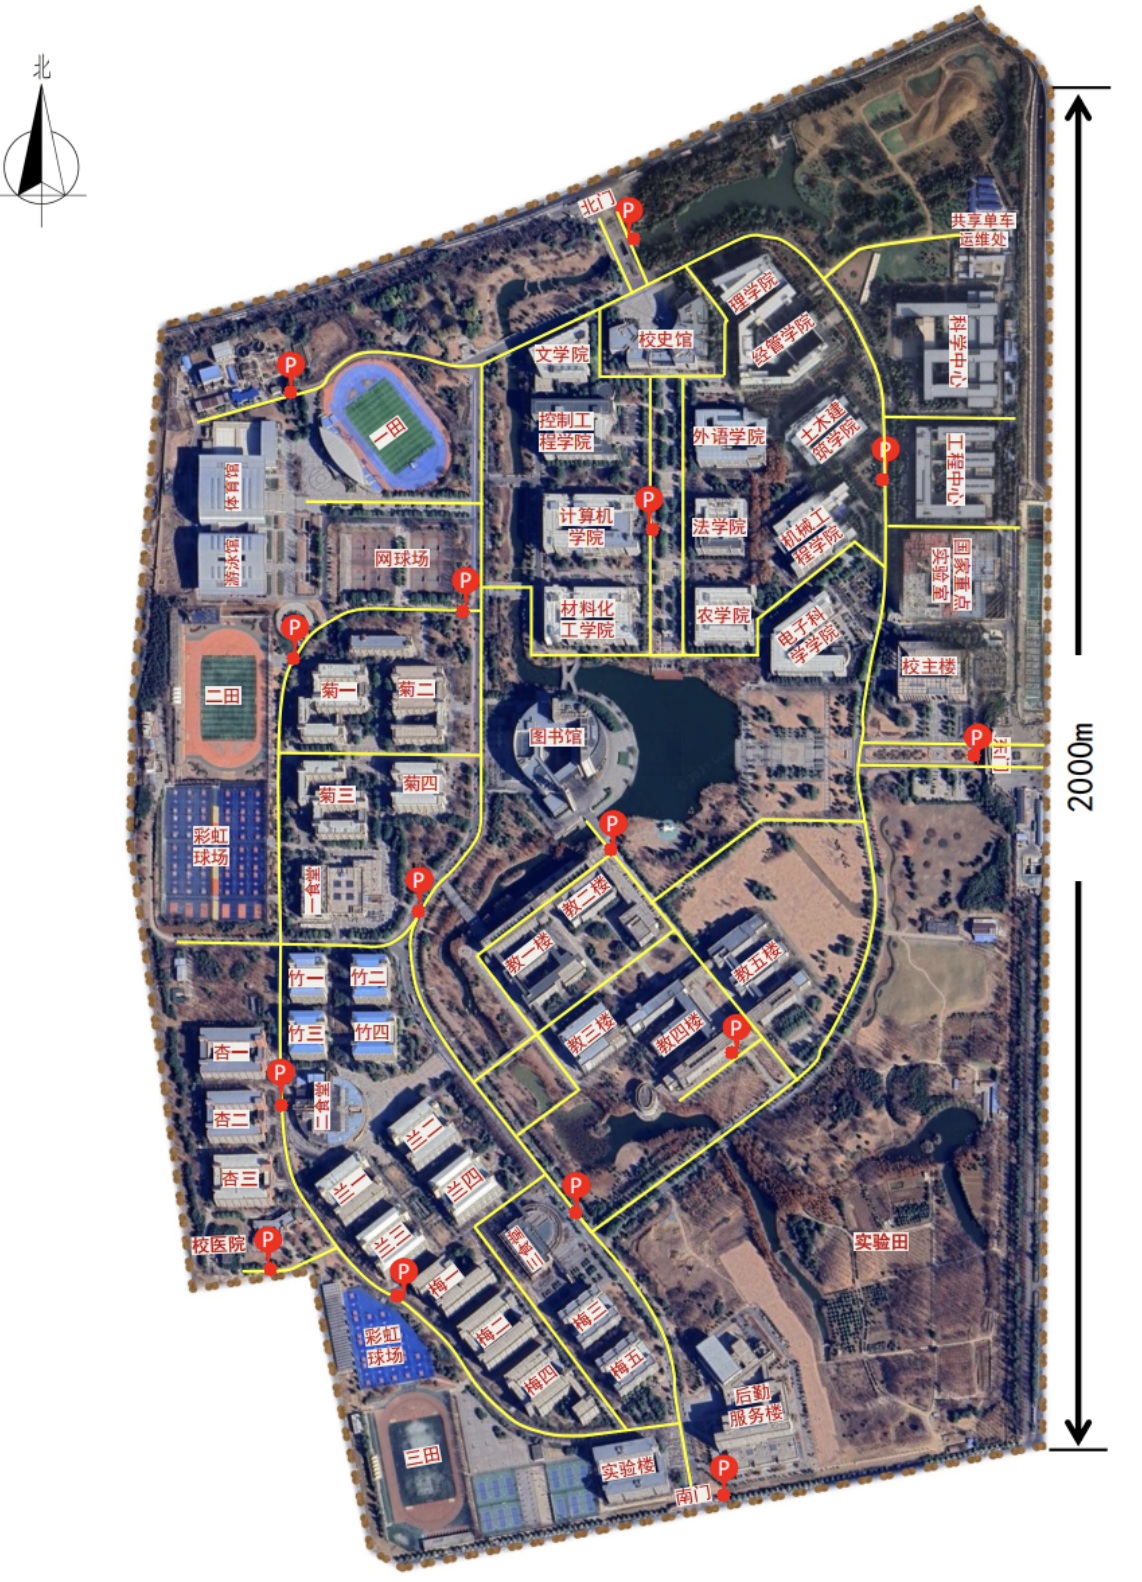
\includegraphics[width=0.45\linewidth]{交互式标注图.jpg}
    }
    \hfill % 水平间距控制
    \subfloat[模拟路径图]{
        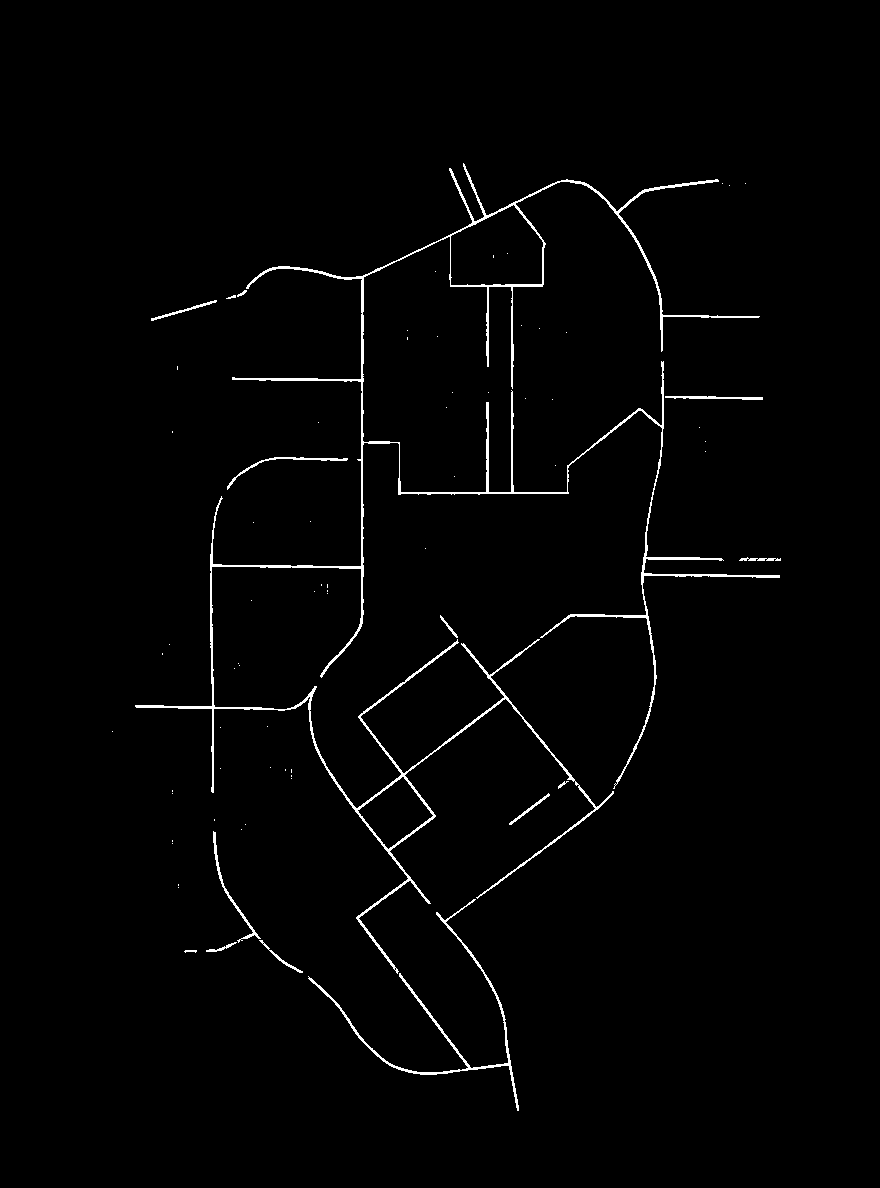
\includegraphics[width=0.45\linewidth]{initial_mask.png}
    }
    \label{fig:side-by-side}
    \caption{交互式标注与模拟路径图}\label{fig:交互式标注与模拟路径图}
\end{figure}

\begin{figure}
    \centering
    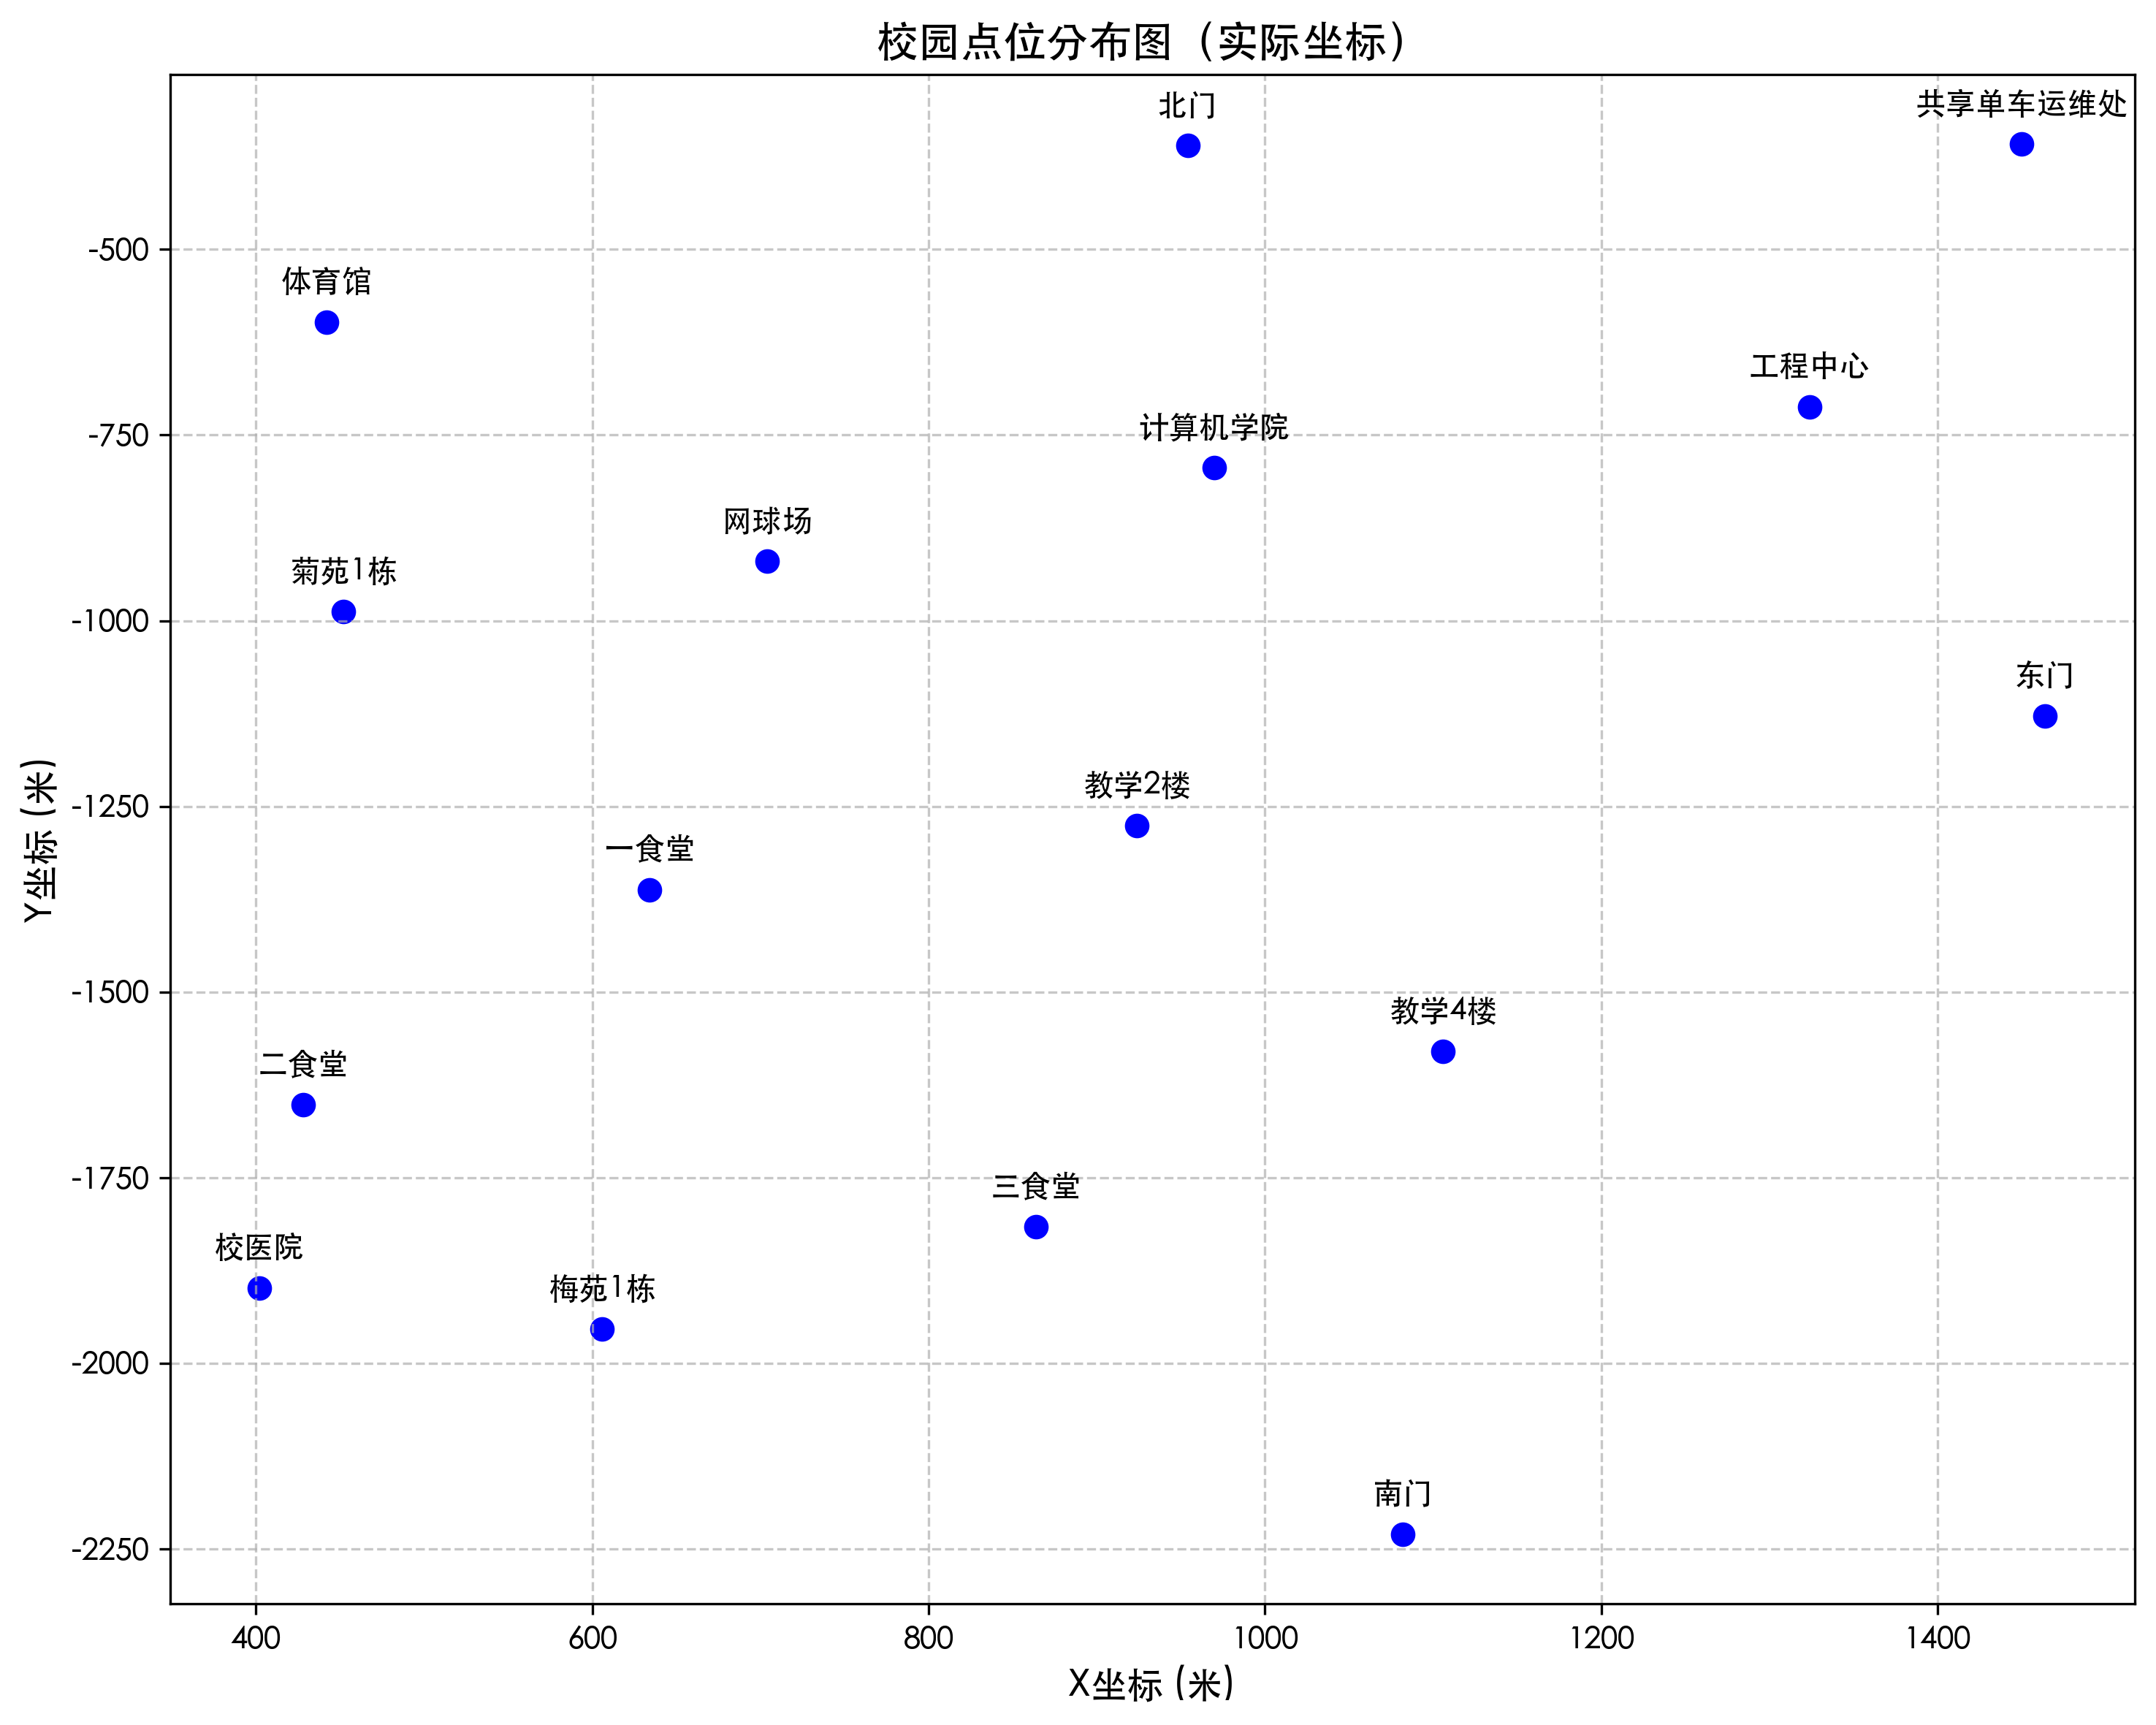
\includegraphics[width=0.75\linewidth]{校园点位分布图_实际坐标.png}
    \caption{真实坐标图}
    \label{fig:enter-label}
\end{figure}

校园内16个地点以二维坐标表示,坐标为 $(x_i, y_i)$,单位为米,构建覆盖校园范围的无向路网图。对于每一停车点,首先定位其在路网中最近的节点位置,然后利用 Dijkstra算法在图中计算两节点之间的最短路径长度,作为两点之间的路网距离:
\begin{equation}
    d_{ij} = \min \left\{ \sum_{(u,v) \in P} w_{uv} \,\middle|\, P \text{ 为 } i \text{ 到 } j \text{ 的路径} \right\}
\end{equation}
其中$w_{uv}$为两节点之间各条路径的长度。

最终构建距离矩阵$D = [d_{ij}]$\label{距离矩阵}用于路线优化。

接下来考虑上一个任务中求得的需求数据,对其进行调整,对于时间段 $[t_s, t_e]$,需求 $q_i$计算如下:
\begin{equation}
    q_i = (n_i(t_e) - n_i(t_s)) \cdot w(t_e), \quad i \in {1, 2, \dots, 15}
\end{equation}
其中 $n_i(t)$为地点$i$在时间$t$的单车数,$w(t_e)$为时间权重,定义为:
\[
w(t_e) = 
\begin{cases}
0.2, & t_e = \text{7:00}, \\
0.4, & t_e = \text{9:00}, \\
1.1, & t_e = \text{12:00}, \\
0.9, & t_e = \text{14:00}, \\
0.6, & t_e = \text{18:00}, \\
0.5, & t_e = \text{21:00}, \\
0.2, & t_e = \text{23:00}.
\end{cases}
\]
运维处需求设为 $q_0 = 0$,正需求 $( q_i > 0 )$表示需要单车,负需求 $( q_i < 0 )$表示单车过剩。

为处理需求超出车辆容量的情况,采用需求拆分策略。若地点 $i$的需求$q_i > 20$或$q_i < -20$,则拆分为多个需求块:
\begin{equation}
    q_i = \sum_{k=1}^{K_i} q_{i,k}, \quad |q_{i,k}| \leq 20
\end{equation}
其中正需求拆分为$q_{i,k} \leq 20$,负需求拆分为$q_{i,k} \geq -20$。每个$q_{i,k}$对应虚拟节点$v_{i,k}$,其距离矩阵继承原始节点的距离:
$d_{v_{i,k}, v_{j,l}} = d_{i,j}$。

\textbf{Step2:} \textbf{求解模型}

初始解通过\textbf{贪心策略}构建,将所有虚拟节点按需求绝对值$|q_i|$降序排列,再按轮询方式为每辆车分配节点,构建行程$ t = [0, v_1, \dots, v_k, 0]$,并确保满足Step1中设置的四个平衡条件。

对于单一节点行程,若节点需求为正,尝试添加负需求节点以平衡负载(反之亦然)。据此得到的初始解的总时间为:
\begin{equation}
    T_{\text{initial}} = \sum_{v=1}^{V} \sum_{t \in \text{Trips}_v} \frac{D(t)}{s} \cdot 3600
\end{equation}\par
算法以一个可行的初始解作为起点,设置初始温度 $T_0 = 1000$,最小温度阈值为$T_{\min} = 1$,温度每次迭代按冷却系数 $\alpha = 0.99$ 缓慢降低。在每一温度层,固定迭代次数为$I = 100$。

为提升解空间的搜索能力,本文在\textbf{模拟退火过程中引入了两类邻域操作}:交换(Swap)与移动(Move)。交换操作通过在两辆车的行程中随机选取两个中间节点并进行互换,从而调整各自的调度顺序;移动操作则是在一条行程中随机选择一个中间节点,并将其插入另一辆车的某个行程中,以改变节点分布。上述两种操作均能在保持解结构基本稳定的同时实现局部扰动,有效扩展搜索空间。

每一次邻域扰动后,需对新生成的调度方案进行\textbf{可行性验证},主要包括两方面的约束:一是容量约束,即车辆在任何时间点的负载应为非负且不超过其最大承载量(本模型中为20辆);二是时间约束,即单次调度行程及每辆车的总调度时间均不得超过给定上限(设定为7200秒)。只有在同时满足上述两个约束条件的前提下,扰动后的新解才会被视为可接受的候选方案。

在具体执行中,当前解 S 的成本(即调度总时间)记作 C(S),每次迭代中,通过随机选择邻域操作生成新解 ${\prime}$。若 $S{\prime}$ 可行,则计算其相对当前解的成本变化 $\Delta C = C(S{\prime}) - C(S)$。若新解成本更低,则直接接受该解;若成本上升,则以概率 $e^{-\Delta C / T}$ 接受次优解,从而有效跳出局部最优陷阱。在整个降温过程中,若发现更优解 $S_{\text{best}}$,则及时记录作为当前最优解。最终,当温度低于 $T_{\min} $时,算法终止,返回所找到的最优调度方案。


\begin{figure}[H]
\centering
\subcaptionbox{12:00-14:00 运维车调度模拟直线图\label{fig:12:00-14:00 运维车调度模拟直线图}}
{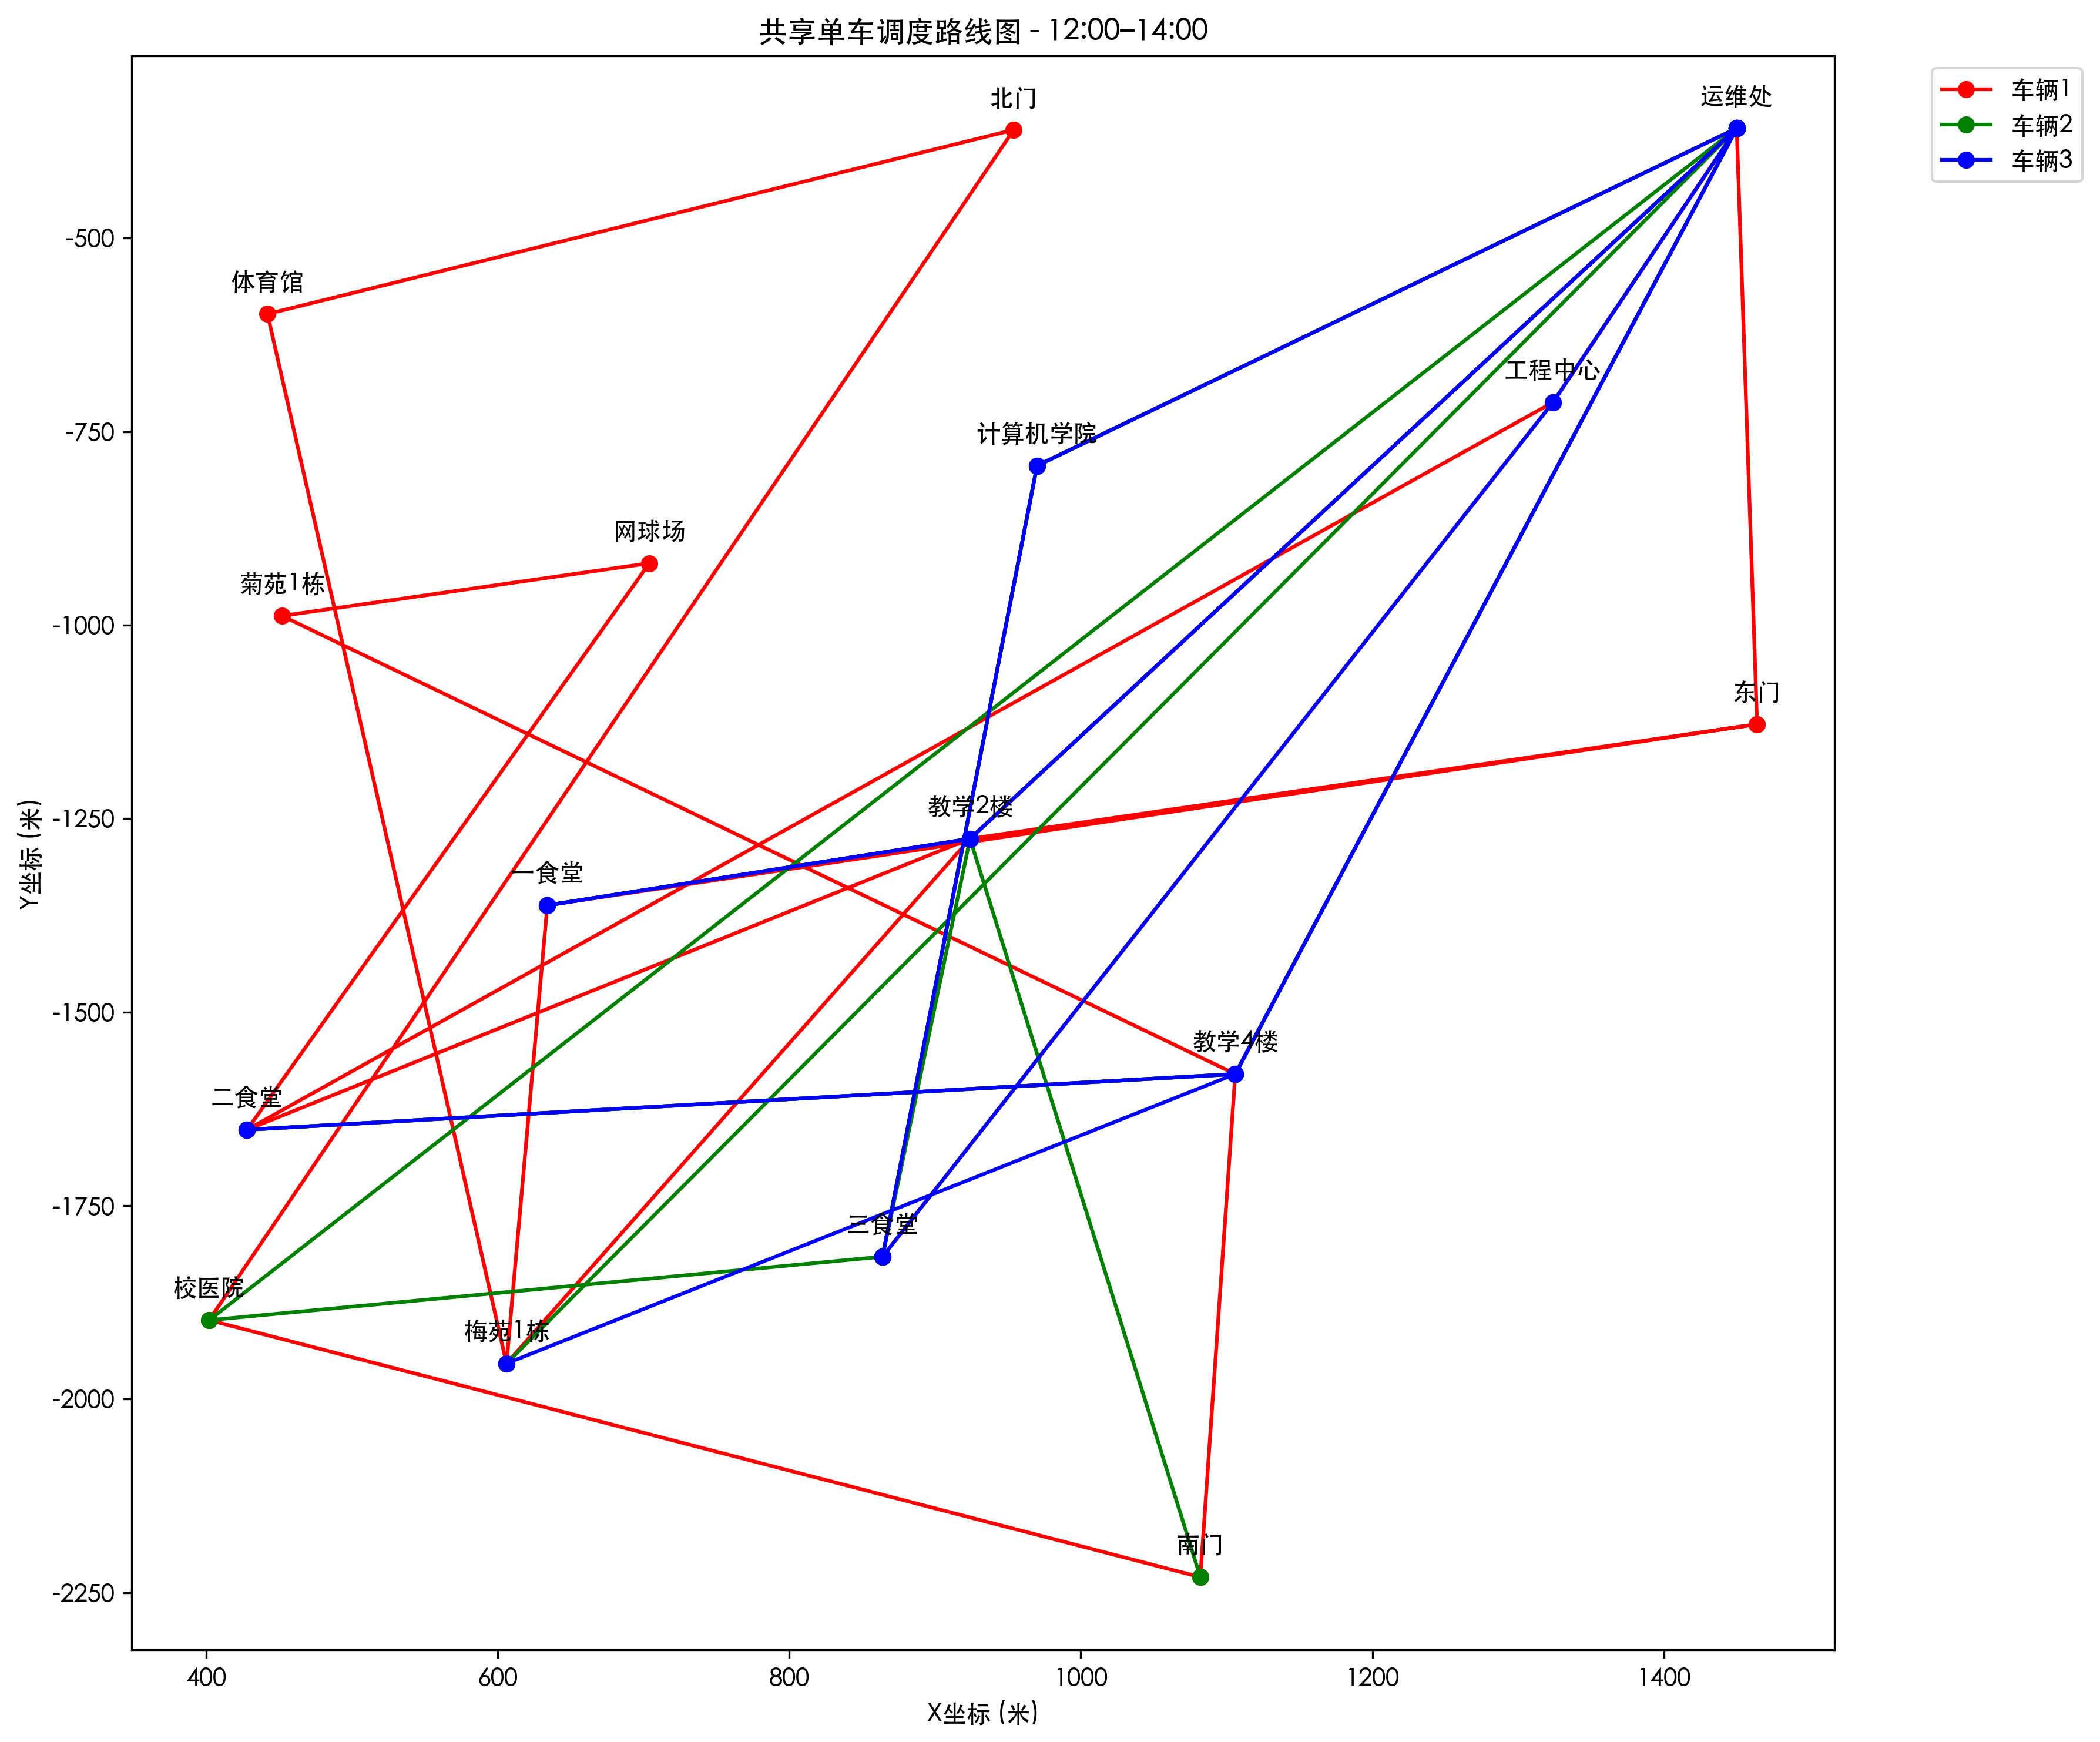
\includegraphics[width=.45\textwidth]{问题2-调度路线图-12:00-14:00.png}}
\subcaptionbox{高峰期运维车调度弦图\label{fig:高峰期运维车调度弦图}}
{\includegraphics[width=.45\textwidth]{2821745116442_.pic.jpg}}
\caption{运维车调度图}\label{fig:运维车调度图}
\end{figure}

\textbf{Step2:} \textbf{结果分析}

为验证所提出 CVRPTC-SA 算法在校园共享单车调度问题中的适用性与有效性,本文选取早高峰、中午、晚高峰等六个典型时间段,分别独立运行算法并生成调度方案。由于篇幅限制,文中以12:00-14:00时间段为例展示算法的典型输出结果(为提升算法的鲁棒性,以下数值基于多次模拟的平均结果,考虑了随机扰动可能带来的轻微波动)。

\begin{figure}[H]
  \centering
  \includegraphics[width=0.8\linewidth]{ac4cf9fe255b2adab439ba7d560f2db9.png} % 图片路径
  \caption{12:00-14:00运维车调度路线图} 
  \label{fig:7:00-9:00运维车调度路线图}
\end{figure}

在该时间段中,虚拟节点的需求覆盖了校园内多个区域,包含若干正负需求点。经模拟退火优化后,算法输出了多辆调度车辆的行驶路径示例,涵盖起止点、途经节点序列以及每条路径的距离、耗时与净搬运量,其中,净搬运量为\textbf{363辆},能较好地满足午高峰期教学楼对共享单车的大量需求。


\section{问题三\hspace{1em}运营效率评价模型与点位布局调整}
\subsection{问题三分析}
问题三要求建立共享单车运营效率的评价模型,并依此判断是否要调整校内停车点位布局。沿用问题二中的定义,本文构建了基于\textbf{线性规划}的点位优化模型,在初始库存、流量平衡、需求满足、调度容量和正需求点参与的约束条件下,结合调度效率、需求满足率和点位利用率三大效率维度,利用\textbf{Gurobi}分别计算并比较初始点位和变化点位的的综合运营效率,进而判断校内停车点分布的合理性。
\subsection{模型建立}
\textbf{Step1:} \textbf{设置变量与目标函数}

在问题二的基础上扩展,系统包括点位集$P=\{p_1,p_2,\dots,p_{15}\}$、时段集$T=\{T_0,\dots,T_6\}$和\ref{距离矩阵}中的距离矩阵$D = [d_{ij}]$与停车点需求$q_i$,目标是优化共享单车调度量 $x_{ijt}$(从点位$i$到$j$在时段$t$调度的单车数量),以最小化调度时间来满足需求并平衡点位利用率,由此构建的目标函数如下:

\begin{equation}
    \min \sum_{i, j, t} c_{ij} x_{ijt} + \alpha \sum_{i, t} s_{it} + \beta \sum_t (s_{f+, t} + s_{f-, t})
\end{equation}
其中$c_{ij}$为调度单车从$i$到$j$的成本(时间乘以系数,基于距离),$s_{it}$为需求满足的松弛变量,$s_{f+, t}, s_{f-, t}$为流量平衡的松弛变量,$\alpha=20$为需求无法满足的惩罚,$\beta=10^4$为不守调度平衡的惩罚,强迫系统基本守恒。

\textbf{Step2:} \textbf{约束条件}

模型包含以下约束条件:
\begin{itemize}
    \item \textbf{初始库存:} 
    \begin{equation}
        N_{i0} = N_{i, 7:00}, \forall i \in P
    \end{equation}
    即点位 $i $在 $t=0 $的库存等于初始数据
    \item \textbf{流量平衡:}
    \begin{equation}
        N_{it} + \sum_{j \in P, j \neq i} x_{jit} + s_{f+, t} = \sum_{j \in P, j \neq i} x_{ijt} + N_{i,t+1} + \Delta N_{it} + s_{f-, t}, \forall i \in P, t \in T
    \end{equation}
    即点位$ i $在时段$ t $的库存加上流入量和正松弛等于流出量、下一时段库存、净用户需求和负松弛。
    \item \textbf{需求满足:}
    \begin{equation}
        N_{it} + \sum_{j \in P, j \neq i} x_{jit} - \sum_{j \in P, j \neq i} x_{ijt} + s_{it} \geq D_{it}, \forall i \in P, t \in T
    \end{equation}
    即库存加净流入量加上松弛量需满足正需求。
    \item \textbf{调度容量:}
    \begin{equation}
        80 \leq \sum_{i \in P} \sum_{j \in P, j \neq i} x_{ijt} \leq 600, \forall t \in T
    \end{equation}
    \item \textbf{正需求点参与:}
    净需求大于50的点位必须参与调度
\end{itemize}

\subsection{模型求解}
将上述目标函数和约束条件输入\textbf{线性规划求解器Gurobi},从调度时间、用户需求满足程度及点位资源配置均衡性三个维度出发,通过下列指标评估运营效率:
\begin{description}
    \item[调度效率 ] 最大调度时间减去实际时间后归一化,反映在单位最大调度时间下,实际完成任务所需时间的节省比例
    \begin{equation}
        S_{e} = (129600 - T_{total}) / 129600, T_{total} = \sum_{t \in T} \sum_{i \in P} \sum_{j \in P, j \neq i} c_{ij} x_{ijt}
    \end{equation}
    \item[需求满足率 ] 用于衡量实际可提供车辆数是否满足用户需求
    \begin{equation}
        D_{s} = (\frac{1}{|P||T|}) \sum_{i \in P} \sum_{t \in T} min(1, \frac{N'_{it}}{D_{it}}) * 100, N'_{it} = N_{it} + \sum_{j \in P, j \neq i} x_{jit} - \sum_{j \in P, j \neq i} x_{ijt}
    \end{equation}
    \item[点位利用率 ] 反映系统中各点位的总需求在整体需求中的分布均衡程度
    \begin{equation}
    U = \frac{1}{|P|} \sum_{i \in P} \left( \frac{d_i}{d_{\max}} \right) \times 100
    \end{equation}
    其中, $d_i = \sum_{t \in T} \Delta N_{it}$  表示点位$  i  $在所有时段的总需求量, $d_{\max}$  为所有点位中最大总需求。
\end{description}

通过对上述三大效率评估指标进行加权平均,我们最终确定了共享单车运营效率的评估公式,具体如下:

\begin{equation} 
    E = 0.4 \times S_{\text{e}} + 0.3 \times \left(\frac{D_{\text{s}}}{100}\right) + 0.3 \times \left(\frac{U}{100}\right)
\end{equation}
\subsection{结果分析}
基于上述分析,计算出\textbf{初始运营效率为0.7392},不足以解决高峰期共享单车的供需矛盾,故原点位设置存在\textbf{不合理}之处。通过不断优化点位布局,运营效率有所上升,选取\textbf{优化效果最佳的点位调整方案}得:优先移除校医院和体育馆点位,新增坐标$(798.23, -1494.76)$的教学食堂结合新区点位和坐标$(668.72,-601.53)$的一田右侧点位,可将综合运营效率提升至\textbf{0.8588},相较于初始点位提升\textbf{16.18\%},点位分布如下图所示:
其中,红点为新增停车点位,星号标注为建议去除点位。
\begin{figure}
    \centering
    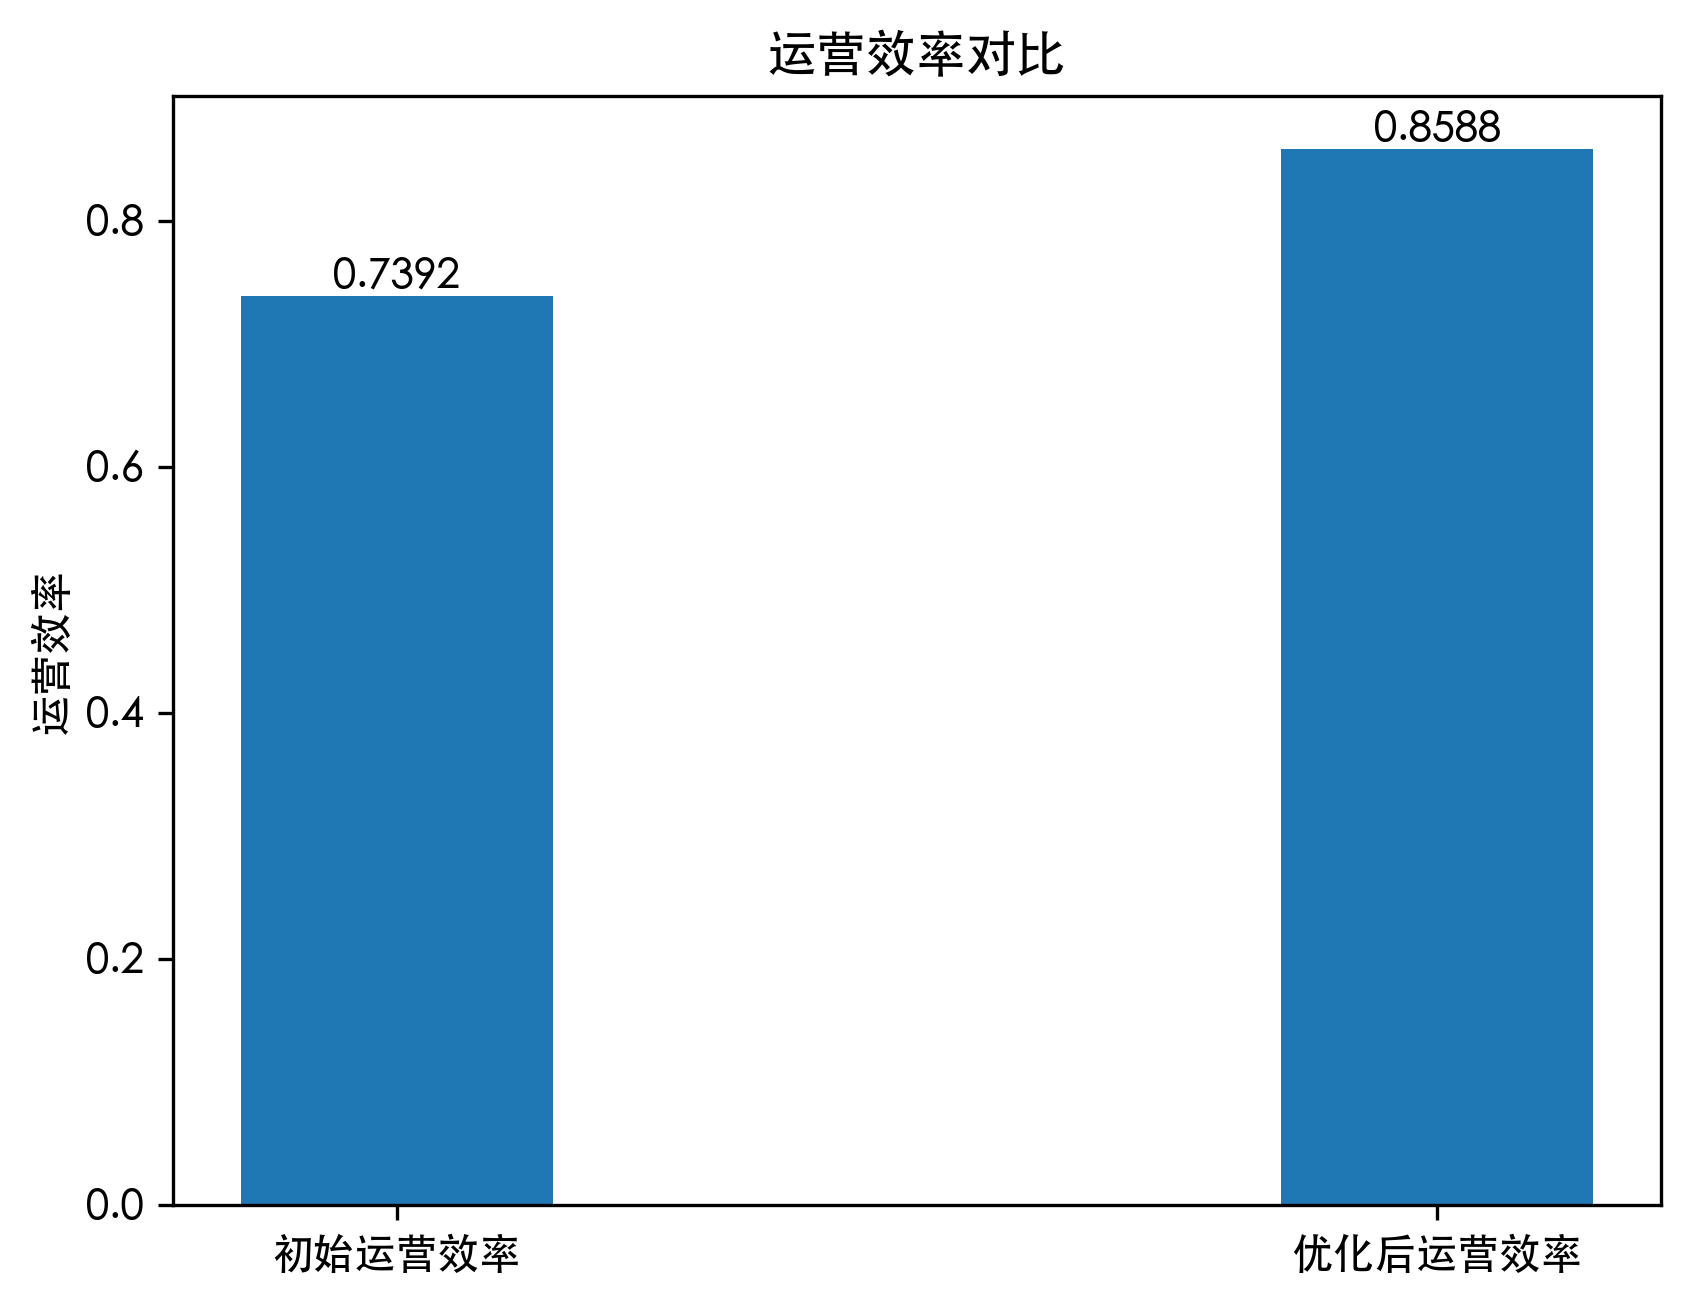
\includegraphics[width=0.5\linewidth]{运营效率对比图.png}
    \caption{运营效率对比图}
    \label{fig:enter-label}
\end{figure}

\begin{figure}[H]
  \centering
  \includegraphics[width=0.8\linewidth]{11731745116987_.pic.jpg} % 图片路径
  \caption{点位分布图(新)} 
  \label{fig:点位分布图(新)}
\end{figure}



%%%%%%%%%%%%%%%%%%%%%%%%%%%%%%%%%%%%%%%%%%%%%%%%%%%%%%%%%%%%% 

\section{问题四\hspace{1em}维修巡检调度模型}
\subsection{问题四分析}
沿用问题二的处理方式,在已经建立的\textbf{CVRPTC-SA}模型之上进行调整:
\begin{description}
    \item[步骤一] 构建停车点集  $P = \{1, 2, \dots, n\}$ ,设每个点  $i \in P $ 有故障车辆数量  $d_i $,检修车辆集为 $ V $,平均处理一辆车需时  $t_p $ 分钟。车辆从维修中心出发,访问若干点后返回。
    \item[步骤二] 修改约束条件,构造目标函数最小化所有车辆调度路径总耗时。
    \item[步骤三] 贪心策略生成初始解,采用交换和移动操作生成邻域解,设置模拟退火参数后进行迭代。
    \item[步骤四] 绘制车辆调度路径图。

\end{description}
\subsection{模型求解与结果分析}
与问题二相比,模型的车辆容量和车辆速度不变,需要修改的约束条件如下:
\begin{itemize}
    \item \textbf{回收数不能超过故障数:}
    \begin{equation}    
    y_i^v \leq r_i, \quad \forall i \in P, v \in V
    \end{equation}
    其中$y_i^v$为运维车在$P=i$处回收的故障车辆,$r_i$为该处故障车辆总数。
    \item \textbf{路径连续性(流平衡约束):}
    \begin{equation}    
    \sum_{j \in P, j \neq i} x_{ij}^v = \sum_{j \in P, j \neq i} x_{ji}^v, \quad \forall i \in P, v \in V
    \end{equation}
    
\end{itemize}

下面图\ref{fig:运维车巡检图}展示的是在故障车辆数为\textbf{57辆}(占总数6\%)时三辆运维检修车的行驶路线图。图中两点间直线长度实际代表两点的路网距离。
\begin{figure}[H]
  \centering
  \includegraphics[width=0.6\linewidth]{2881745121878_.pic.jpg} % 图片路径
  \caption{运维车巡检图} 
  \label{fig:运维车巡检图}
\end{figure}

\begin{table}[H]
\centering
\caption{运维车巡检路线与时间表}
\label{tab:运维车巡检路线与时间表}
\begin{tabular}{|c|p{5cm}|c|c|c|c|}
\hline
\textbf{行程编号} & \textbf{巡检路线} & \textbf{行驶时间 (秒)} & \textbf{搬运时间 (秒)} & \textbf{总时间 (秒)} & \textbf{搬运车辆 (辆)} \\
\hline
行程 1 & 运维处 $\to$ 三食堂 $\to$ 教学食堂结合新区 $\to$ 二食堂 $\to$ 运维处 & 569 & 1200 & 1769 & 20 \\
\hline
行程 2 & 运维处 $\to$ 一食堂 $\to$ 二食堂 $\to$ 北门 $\to$ 梅苑1栋 $\to$ 运维处 & 933 & 1200 & 2133 & 20 \\
\hline
行程 3 & 运维处 $\to$ 菊苑1栋 $\to$ 南门 $\to$ 教学2楼 $\to$ 梅苑1栋 $\to$ 东门 $\to$ 教学4楼 $\to$ 运维处 & 1055 & 1020 & 2075 & 17 \\
\hline
\end{tabular}
\end{table}

由表\ref{tab:运维车巡检路线与时间表}中结果可得,\textbf{行程 1 仅用时 1769 秒即完成 20 辆故障车辆的回收任务,单车平均耗时仅为 88.45 秒,运力利用率和调度效率均达到最优。}这说明模型在路径规划过程中充分考虑了点位分布与路径连通性,能够智能优先选择回收密集度较高、路径连通性良好的点位,从而大幅缩短调度周期。

行程 2 虽然行驶时间较长(933 秒),但仍实现了满载回收,验证了\textbf{模型在复杂路径下仍具备较强的适应能力与路径优化能力}。相较之下,行程 3 搬运车辆数为 17,虽未达到最大运载能力,但在约束条件下仍合理安排了巡检次序,总耗时控制在 2075 秒以内,展现了\textbf{模型对非均衡需求区域的灵活调度能力}。

总体而言,CVRPTC-SA 模型不仅能生成满足现实约束条件的高效路径,而且在任务分配、车辆调度和路线安排等方面均展现出高度智能化和适应性。通过模拟退火的全局优化能力与 Dijkstra 最短路径算法的高效结合,模型成功实现了“在有限时间内最大限度回收故障车辆”的调度目标,为共享单车系统的智能化运维提供了可推广的算法支持和实践路径。
%%%%%%%%%%%%%%%%%%%%%%%%%%%%%%%%%%%%%%%%%%%%%%%%%%%%%%%%%%%%%

\section{模型的评价与改进}

\subsection{模型评价}

首先,在准确性方面,问题一通过最小二乘法结合 K-means 聚类方法估算单车总量,得到最终估算值为 972 辆,相比初始估算值 961 辆提升了稳定性,聚类后的调整因子有效捕捉了不同时间段的流动性特征,模型收敛性良好。问题二采用 XGBoost 算法预测用车需求,$R^2$ 和 RMSE 指标显示其预测精度优于 LightGBM 和线性回归模型,尤其在高峰时段表现出较强的非线性拟合能力。问题三的运营效率评价体系综合了调度效率、需求满足率和点位利用率,优化后综合效率从 0.7392 提升至 0.8588,表明点位调整方案有效改善了供需平衡。问题四的巡检调度模型基于 CVRPTC-SA 算法,最优调度方案成功将6\%的故障车辆比例全部运回修理,验证了模型在故障车辆清理中的高效性。

其次,在实用性方面,新增教学食堂结合新区和一田右侧点位,移除校医院和体育馆点位,调整方案直接提升了 16.18\% 的运营效率,为校园单车管理提供了可执行的决策支持。

最后,在鲁棒性方面,模型对数据缺失和分布不均的处理较为稳健。问题一通过时间一致性和停车点相似性补全缺失值,并采用三次样条插值方法平滑时间序列数据,确保了分布估算的连续性。然而,模型仍存在一定局限性:问题一和问题二对周末数据的权重较低,可能忽略了周末用车模式的特殊性;问题四的巡检模型未充分考虑故障车辆分布的动态变化,可能影响长期调度效率。
\subsection{模型改进}

对于问题三的点位优化模型,可引入多目标优化框架。未来可引入步行距离约束,通过 Pareto 优化方法平衡效率与用户体验,生成更贴近实际需求的点位布局方案。

最后,对于问题四的巡检调度模型,建议引入故障车辆的动态预测机制。可结合历史故障数据和环境变量(如降雨、温度),通过时间序列模型(如 ARIMA)预测各时段故障分布,并动态调整巡检路线和时间,从而进一步缩短总调度时间,提高故障清理效率。
%%%%%%%%%%%%%%%%%%%%%%%%%%%%%%%%%%%%%%%%%%%%%%%%%%%%%%%%%%%%%


%%%%%%%%%%%%%%%%%%%%%%%%%%%%%%%%%%%%%%%%%%%%%%%%%%%%%%%%%%%%%
%% 参考文献
\nocite{*}
\bibliographystyle{gbt7714-numerical}  % 引用格式
\bibliography{ref.bib}    
% ref.bib
\newpage
%%%%%%%%%%%%%%%%%%%%%%%%%%%%%%%%%%%%%%%%%%%%%%%%%%%%%%%%%%%%%
%% 附录
\begin{appendices}
\section{问题一 表1}

\begin{table}[H]
\centering
\large % 增大字体为 \large
\renewcommand{\arraystretch}{1.5} % 行间距设为 1.5 倍
\begin{tabularx}{\textwidth}{@{}L *{7}{R}@{}}
\toprule
\multirow{2}{*}{停车点位} & \multicolumn{7}{c}{时间段} \\ 
\cmidrule(lr){2-8}
 & 7:00 & 9:00 & 12:00 & 14:00 & 18:00 & 21:00 & 23:00 \\
\midrule
东门       & 17  & 71  & 32  & 56  & 36  & 103 & 14  \\
南门       & 14  & 130 & 59  & 26  & 110 & 41  & 46  \\
北门       & 2   & 66  & 70  & 66  & 72  & 27  & 28  \\
一食堂     & 73  & 0   & 91  & 0   & 33  & 22  & 82  \\
二食堂     & 141 & 0   & 130 & 0   & 74  & 71  & 114 \\
三食堂     & 109 & 0   & 147 & 0   & 61  & 54  & 123 \\
梅苑1栋    & 130 & 1   & 81  & 12  & 67  & 0   & 128 \\
苑苑1栋    & 136 & 6   & 79  & 68  & 195 & 68  & 126 \\
教学2楼    & 0   & 218 & 52  & 206 & 35  & 109 & 30  \\
教学4楼    & 0   & 150 & 29  & 151 & 26  & 81  & 20  \\
计算机学院 & 0   & 53  & 14  & 88  & 48  & 49  & 17  \\
工程中心   & 0   & 59  & 12  & 78  & 42  & 76  & 49  \\
网球场     & 4   & 20  & 4   & 17  & 48  & 8   & 15  \\
体育馆     & 1   & 2   & 2   & 5   & 34  & 5   & 12  \\
校医院     & 5   & 29  & 6   & 38  & 6   & 7   & 11  \\
\bottomrule
\end{tabularx}
\label{tab:停车点位数量分布(部分)}
\end{table}


\section{代码}
\noindent 
求解真实坐标部分
\lstinputlisting[language=python]{code/question1.py}
\textbf{CVRPTC-SA}算法部分
\lstinputlisting[language=python]{code/question2.py}
\end{appendices}
\end{document}



